\section{Introduction}

Compressed sensing is a novel techniques introduced by Donoho \cite{donoho2006sparse} and by Candes, Romberg, and Tao \cite{candes2006robust} in 2006, and since then has become a key concept in various areas of applied mathematics, computer science, and electrical engineering. It demonstrates that high-dimensional signals that allow a sparse representation through  a suitable basis or, more generally, a frame, can be recovered by using effective algorithms from what was previously considered
highly incomplete linear measurements. This chapter presents
an introduction and a survey of compressed sensing.

\section{Sampling System}

In many real world applications, signals are usually sampled and stored in digital devices for further analysis, such as medical image imaging and CT tomography. From the discrete sampling and storage, the system are expected to be able to exactly reconstruct the original signals using observations as less as possible. 

Assuming that the original signal is $1 \times N$ vector, the observation behaviour can be modelled as a sensing matrix A with a size of $m \times N$. Then the sampled data $y$, an $m \times 1$ vector, can be described as
\begin{equation}
\label{sampling-eq}
y = Ax,
\end{equation}
Then an important question arises:
\begin{itemize}
\item 
In order to reconstruct signal $x$, what is the minimum samples are needed in $y$?
\end{itemize}

Conventional linear algebra theory states that unique solution of (\ref{sampling-eq}) exists only if $m \geq N$. That is to say, at least N samples are needed in $y$. However, consider a case when the signal $x$ is sparse, which means most of the values in $x$ are zero or relatively small, can $x$ be reconstructed using smaller numbers of observations $y$? (i.e. with $m < N$)

Conventionally, if $m < N$, the the equation (\ref{sampling-eq}) is underdetermined, such that multiple possible solutions exist. This means it is not possible to uniquely recover the original signal $x$. 
However, if the $x$ is sparse, then the answer maybe Yes, based on the technique of Compressed Sensing (CS). That is, the CS allows a possible sparse information’s reconstruction from a very few
numbers of samples $y$ ($m << N$).

The sparse characteristics can naturally exist (such
as $x$) or generated by orthogonal basis decomposition (such as $x = As$ where $s$ is sparse, $A$ is the basis e.g. wavelets decomposition). As such, the CS approach provides a feasible method to theoretically reduce the number of observations required. The essence of the CS is hence to :
\begin{itemize}
\item Find the minimum number of samples for the sensing matrix.
\item Design a reconstruction algorithm to uniquely recover original signals via those samples.
\end{itemize}

\section{Sparsity}

Consider a signal $x \in R^{N \times 1}$ which is sparse i.e., it has very few non-zero coefficients in the sense that
\begin{equation}
\label{sparse_eq}
\| x \|_0 := \{i: x_i \neq 0\}
\end{equation}
is small, or that there exists an orthonormal basis $\Psi$ such that $x = \Psi s$, where $x$ is a linear combination of few $k$ basis chosen from $\Psi$, $s$ is the corresponding coefficients of representing $x$ in the domain spanned by the basis $\Psi$. $k$ is then termed as the sparsity.

Naturally, there are many signals directly have sparse information that suitable for the CS based sampling and reconstruction, such as images with low-rank matrix representation, and wireless channels with sparse impulse response coefficients. For those signals who has not apparent sparse structures, it is also possible to derive their approximate sparsity by using orthogonal basis representation or dictionary learning algorithms. As a result, most of physical signals can approximately presents their sparsity in the basis spanned domain and suitable for the CS applications\cite{candes2006robust, candes2006near, rudelson2008sparse, rauhut2012restricted}. In this chapter, it is hence assumed throughout that x is already a sparse vector or can be sparse represented.

\section{Sparse Reconstruction}\label{sct:CS_Recon}

When the $x$ is sparse, an intuitive solution of the underdetermined equation (\ref{sampling-eq}) is equals to the solution of the problem (P0), which aims to find the minimum numbers of supports in $x$ as follows:
\begin{equation}
\label{eq_l0}
P0: \quad min \| x \|_0 \quad s.t. \quad y = Ax
\end{equation}
Then the following Theorem presents the sufficient condition to gain the unique solution:
\begin{theorem}
\label{eq-P0}
Assume that $A \in R^{m \times N}$ is an average of the independent $2k$ column matrix. Then for any $k$-sparse vector $x$, the $x$ can be exactly recovered by solving the problem P0 (\ref{eq_l0}).
\end{theorem}

Hence, according to Theorem \ref{eq-P0}, then there is a coding and decoding of $(A, \Delta)$ such that $x = \Delta(Ax)$, which means $2k$ times the number of observations is sufficient for reconstruction. However, solving the problem P0 is very difficult. In fact, P0 is an NP-complete problem \cite{davis1997adaptive}.

Is there a more efficient decoding algorithms available? The answer maybe Yes if the condition of null space property (NSP) is satisfied (\cite{devore2007deterministic}, Appendix). In this case, using the solution of the following problem P1, which is termed as Basis Pursuit (BP) or l1-norm minimisation, $x$ can be uniquely reconstructed..
\begin{equation}
\label{eq_l1}
P1: \quad min \| x \|_1 \quad s.t. \quad y = Ax
\end{equation}

To solve the problem P1, various types of recovery algorithms exist, such as  convex optimisation and greedy algorithms, where each is having its own advantages and disadvantages. In this section, the widely used linear programming (LP) is used as an example to solve P1:
\begin{equation}
\begin{split}
LP: \quad min \| t_1 + t_2 + \cdots + t_N \|_1 \quad t \in R^N\quad s.t. \quad y = Ax, \\
\quad -t_j \leq x \leq t_j, \quad t_j \geq 0, \quad j = 1 \cdots N
\end{split}
\end{equation}

\todo[inline, color=green!40]{[CH:Mar08]Here I move the details of NSP to the Appendix, because the RIP is the alternative for NSP, and the following discuss of CS recovery are all around the RIP}

\subsection{Restricted Isometry Property}\label{subsct:RIP}

The Section \ref{sct:CS_Recon} and Appendix states that satisfying the NSP condition can enable a more efficient unique reconstruction through solving P1 rather than P0. However, how to verify the sensing matrix $A$ satisfying the NSP condition is computational complex, which render the NSP approach  not practically feasible. A more intuitive concept termed as Uniform Uncertainty Principle, or Restricted Isometry Property (RIP), is introduced in \cite{candes2006robust}. 

%\newtheorem{mydef}{Definition}

%Although the NSP condition presents us an equivalent condition to get unique reconstruction through solving P1, however, how to verify the sensing matrix satisfying NSP in (\ref{nsp-eq}) is computational complex, so NSP is not practically useful.

\begin{mydef}
\label{rip-def}
Let A be an $m \times n$ sensing matrix. Then A has the Restricted Isometry Property (RIP) of order k, if there exists a $\delta_k \in (0, 1)$ such that
\begin{equation}
(1-\delta_k)\|x\|_2 \leq \|Ax\|_2 \leq (1+\delta_k)\|x\|_2 \quad for \; all \; k\; sparse \; x
\end{equation}
\end{mydef}
\begin{theorem}\cite{candes2006robust}
\label{nsp-rip}
A sufficient condition for the null space property (NSP) to hold and for all k-sparse signal is that RIP holds for 2k-sparse signals with
\begin{equation}
\rho = \frac{\sqrt{2} \delta_{2k}}{1-\delta_{2k}} \leq 1
\end{equation}
It follows that if $\delta_{2k} \leq \sqrt{2}-1$ then NSP is satisfied, so that the unique reconstruction can be achieved by l1-norm minimisation (\ref{eq_l1}).
\end{theorem}
According to the Theorem \ref{nsp-rip}, an equivalent condition for the existence of a unique sparse solution of (P1) can now be stated in terms of RIP. If the sensing matrix satisfies the RIP with the $\delta_{2k} \leq \sqrt{2}-1$, then for any k-sparse vector $x$, the Euclidian distance of projected x ( i.e. Ax ) and x still keep very close since the $\delta_{2k} \in (0,1)$ is relatively small.





\begin{figure}[tbh]
\begin{center}
\noindent
  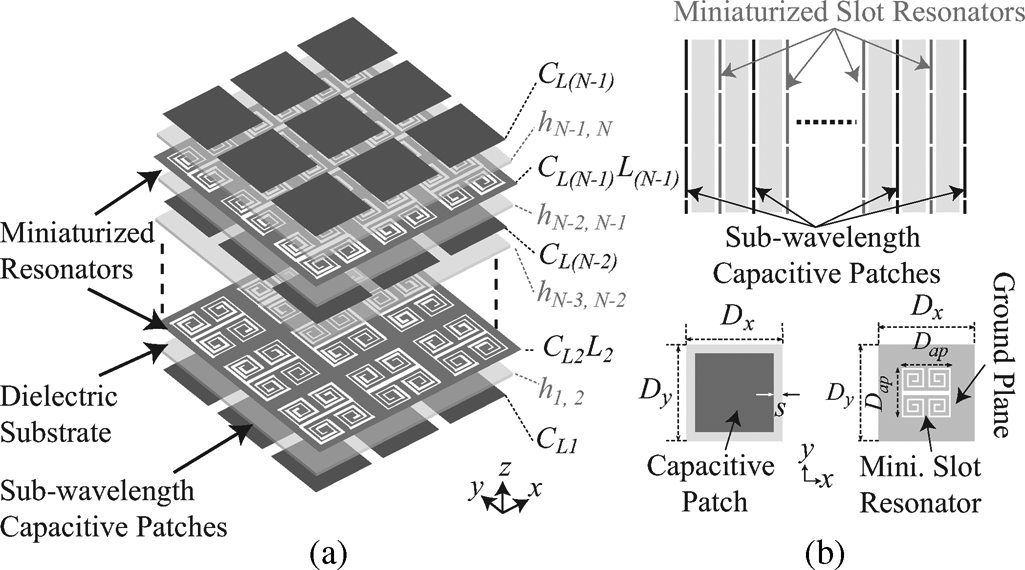
\includegraphics[width=0.7\textwidth]{FigureA}
  \end{center}
    \caption{FigureA's caption.}\label{FigureA}
\end{figure}

Bla bla..

\begin{figure}[tbh]
\begin{center}
\noindent
  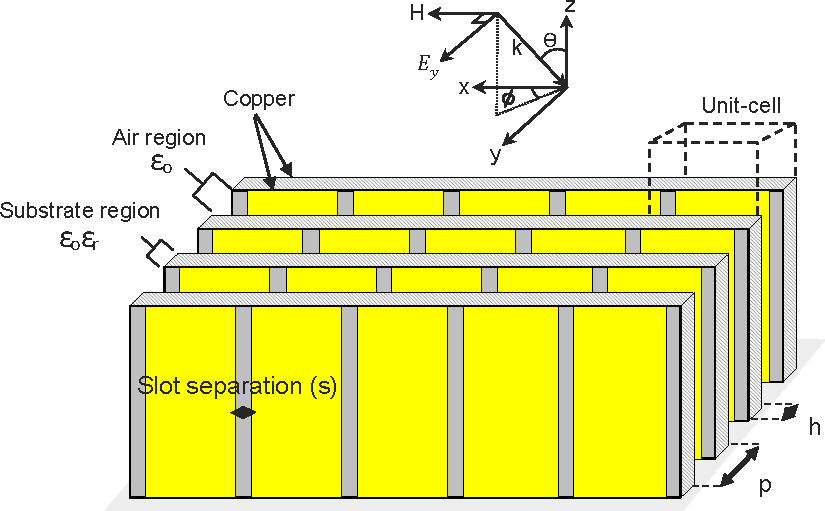
\includegraphics[width=0.7\textwidth]{FigureB}
  \end{center}
    \caption{FigureB's caption.}\label{FigureB}
\end{figure}

\section{Conclusion}

In conclusion, everything has been bla bla all over.
